%#######################################################################
%
% Introduction and motivation for open tool support and VDM + UML
%
\section{Introduction}
%-----------------------------------------------------------------------
%
% Motivation
%
\frame
{
 \frametitle{Motivation}
%\begin{center}
  \begin{itemize}[<+->]
\itemsep=1cm
  \item<1-> Best of both by combining VDM and UML.
  \item<2-> Limited tool support.
  \item<3-> Provide an easy to use and extensible user interface.
  \end{itemize}
%\end{center}
}

%
% Motivation combining knowlage
%
\frame
{
\frametitle{Communication}
  \begin{itemize}
	\itemsep=1cm
  		\item<1-> Formal Method (VDM)
  		\item<2-> Unified Modeling Language (UML)
  		\item<3-> Provide a brother platform of information sharing
  \end{itemize}

}

\note
{

  \begin{itemize}
	%\itemsep=1cm
  		\item Use a formal method to exactly specify what the system should do and prove that it does so.
  		\item Use UML to communicate to domain experts, thus a larger number of people can verify the model.
  		
  \end{itemize}



}

%
% Goal
%
\frame
{
  \frametitle{Goal}

\begin{center}

	\begin{block}<+->{Transformation}
	Provide a connection between VDM and UML. Including UML Class and Sequence Diagrams
	\end{block}
\vspace{1cm}
	\begin{block}<+->{Availability, Extendibility}
	Provide a open source easy to use extensible interface
	\end{block}
%  \begin{itemize}
%	%\itemsep=1cm
%  		\item Provide a connection between VDM and UML
%  		\item Display a VDM static structure diagram (Class Diagram)
%  		\item Creation of Combinatorial Test statements from a dynamic diagram (Sequence Diagram)
%  		\item Integrate the transformation tool into Eclipse
%  		\item Open source
%	  	
%  \end{itemize}
\end{center}
}


%-----------------------------------------------------------------------
\subsection{Vienna Development Method}
%-----------------------------------------------------------------------
%
% VDM
%
\frame
{
  \frametitle{The Vienna Development Method}


	\begin{block}<+->{Not created yet}
	Some thing about VDM
	\end{block}

  \begin{itemize}
	%\itemsep=1cm
  		\item VDM Specification Language (VDM-SL) ISO released in '96
  		\item Extended in 1992-94 with object oriented structure and concurrency handling (VDM++).
  		\item Last extension made for distributed real-time systems (VICE).
  		\item Two most significant tool suites. (VDM Tools and Overture)
	  	
  \end{itemize}


}

%
% Small VDM example
%
\frame
{
  \frametitle{VDM Train example}

\begin{center}

\vdmSpecLineNum{ClassDiagramOverview.vpp}{VDM classes with collections.}{VDM:Collections}

\end{center}
}

%-----------------------------------------------------------------------
\subsection{Unified Modeling Language}
%-----------------------------------------------------------------------
%
% UML
%
\frame
{
  \frametitle{Unified Modeling Language - UML}

\begin{center}

	\begin{block}<+->{Not created yet}
	Some thing about UML
	\end{block}

\end{center}
}


%
% Class Diagram
%
\frame
{
  \frametitle{Class Diagram}

\begin{center}

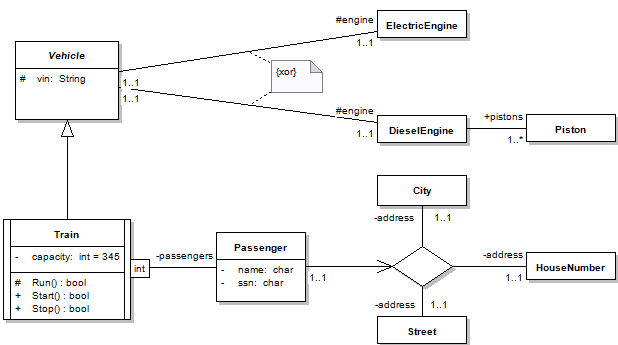
\includegraphics[width=\textwidth]{images/ClassDiagramOverview.png}

\end{center}
}

%
% Sequence Diagram
%
\frame
{
  \frametitle{Sequence Diagram}

	\begin{block}<+->{Needs update}
	This diagram is not the correct one
	\end{block}
\begin{center}
\includegraphics<1->[width=0.5\textwidth]{images/TracesSequenceDiagramEx2.png}%
\end{center}
}
